\section{Mechanical Project}

%%%%%%%%%%%%%%%%%%%%%%%%%%%COLOCAR OS DADOS REAIS DO NOSSO ROB              %%%%%%%%%%%%%%%%%%%%%%%%
In compliance with the SSL rules, the height of the robot is 148 mm, the maximum
percentage of ball coverage is 15\% and the maximum projection of the robot on the ground is 175 mm.
%%%%%%%%%%%%%%%%%%%%%%%%%%%COLOCAR OS DADOS REAIS DO NOSSO ROB              %%%%%%%%%%%%%%%%%%%%%%%%

With the aid of CAD software (Computer Aided Design) and CAM (Computer Aided
Manufacturing) a new robot has been developed. Figure \ref{mec} shows mechanical
3D view and real view of the robot. Shelf had been used allows omnidirectional
movement and has a greater torque that couples the fourth motors (one for each
wheel) for the movement.

\begin{figure}[thpb]
	\centering
	\subfigure[]{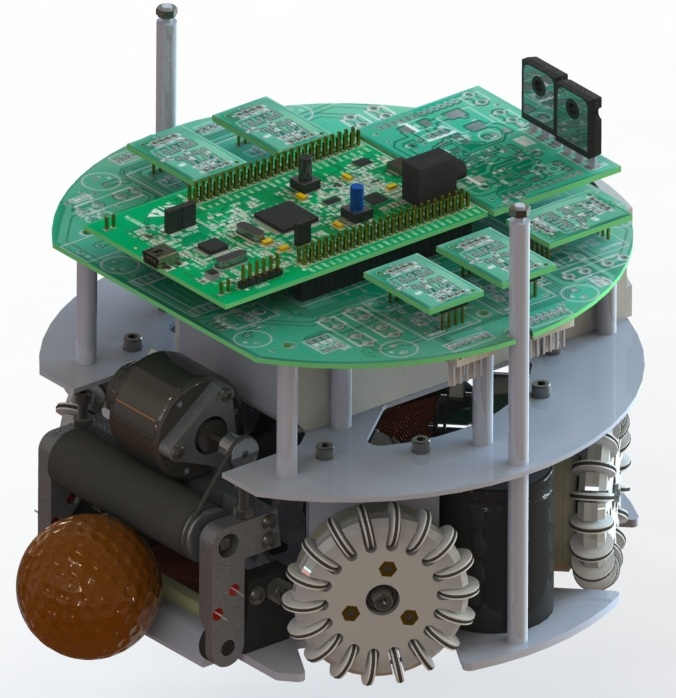
\includegraphics[width = 0.425 \textwidth]{img/cad.jpg}}
	\subfigure[]{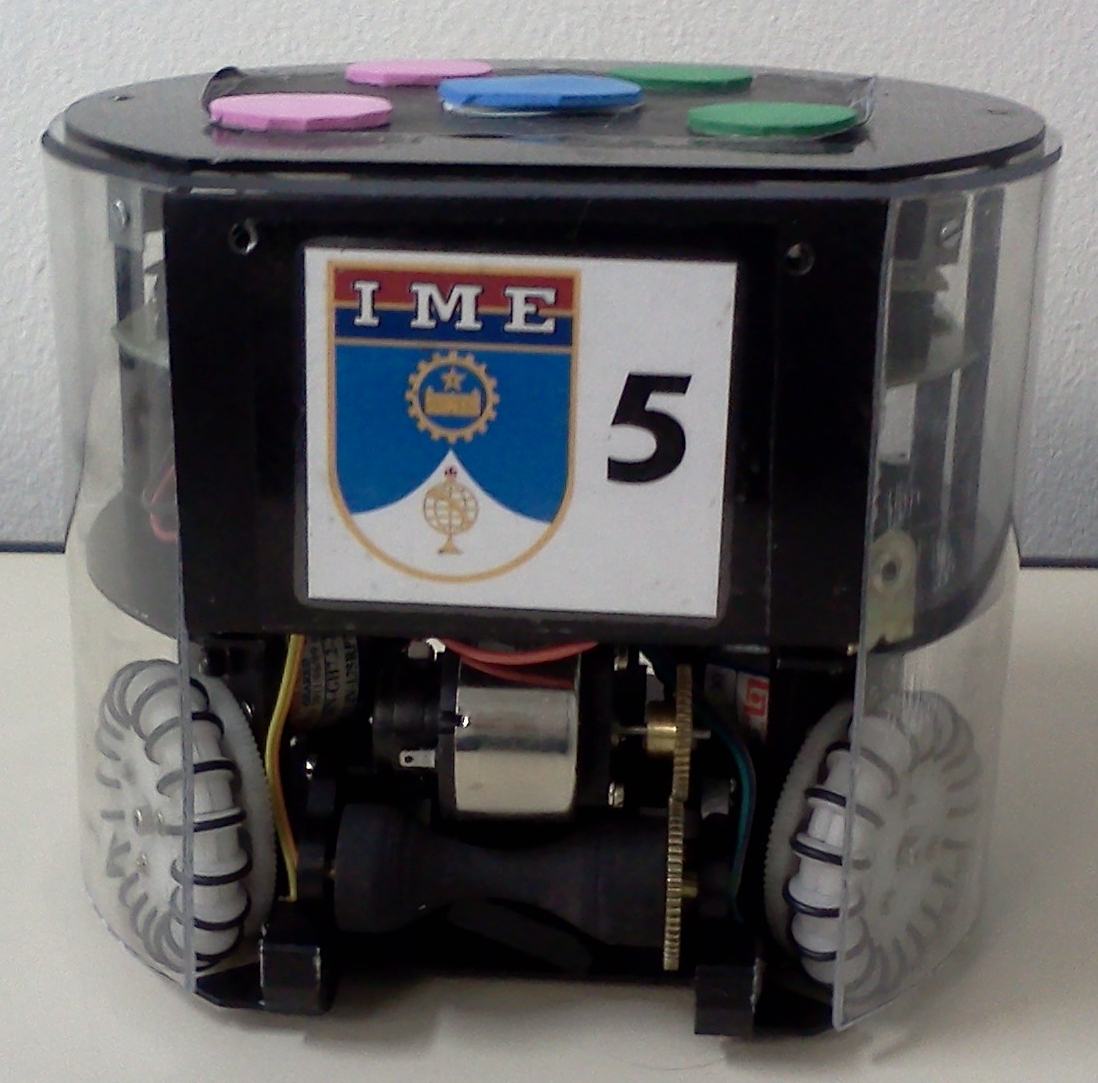
\includegraphics[width = 0.4 \textwidth]{img/robo.jpeg}}
	\caption{(a) Mechanical 3D model view. (b) Robot view.}
	\label{mec}
\end{figure}

The changes in the original design of the model provides a lower weight to
the robot, such as: changing the steel shaft by a shaft of high-strength
aluminium wheels and replacement of aluminium by plastic wheels Polytec
1000. This new design also enables more devices to be shipped. It presents
a diameter of 175 mm and an upper base with holes which give versatility
to the coupling. The fairing of the robot was made from polyvinyl plates.

